% #######################################
% ########### FILL THESE IN #############
% #######################################
\def\mytitle{Coursework Report}
\def\mykeywords{Napier, SET09117, Algorithms, Data Structure, Steven, Gibson, 40270320, Steven Gibson, report}
\def\myauthor{Steven Gibson}
\def\contact{40270320@live.napier.ac.uk}
\def\mymodule{Module Title (SET09117)}
% #######################################
% #### YOU DON'T NEED TO TOUCH BELOW ####
% #######################################
\documentclass[10pt, a4paper]{article}
\usepackage[a4paper,outer=1.5cm,inner=1.5cm,top=1.75cm,bottom=1.5cm]{geometry}
\twocolumn
\usepackage{graphicx}
\graphicspath{{./images/}}
%colour our links, remove weird boxes
\usepackage[colorlinks,linkcolor={black},citecolor={blue!80!black},urlcolor={blue!80!black}]{hyperref}
%Stop indentation on new paragraphs
\usepackage[parfill]{parskip}
%% Arial-like font
\IfFileExists{uarial.sty}
{
    \usepackage[english]{babel}
    \usepackage[T1]{fontenc}
    \usepackage{uarial}
    \renewcommand{\familydefault}{\sfdefault}
}{
    \GenericError{}{Couldn't find Arial font}{ you may need to install 'nonfree' fonts on your system}{}
    \usepackage{lmodern}
    \renewcommand*\familydefault{\sfdefault}
}
%Napier logo top right
\usepackage{watermark}
%Lorem Ipusm dolor please don't leave any in you final report ;)
\usepackage{lipsum}
\usepackage{xcolor}
\usepackage{listings}
%give us the Capital H that we all know and love
\usepackage{float}
%tone down the line spacing after section titles
\usepackage{titlesec}
%Cool maths printing
\usepackage{amsmath}
%PseudoCode
\usepackage{algorithm2e}

\titlespacing{\subsection}{0pt}{\parskip}{-3pt}
\titlespacing{\subsubsection}{0pt}{\parskip}{-\parskip}
\titlespacing{\paragraph}{0pt}{\parskip}{\parskip}
\newcommand{\figuremacro}[5]{
    \begin{figure}[#1]
        \centering
        \includegraphics[width=#5\columnwidth]{#2}
        \caption[#3]{\textbf{#3}#4}
        \label{fig:#2}
    \end{figure}
}

\lstset{
	escapeinside={/*@}{@*/}, language=C++,
	basicstyle=\fontsize{8.5}{12}\selectfont,
	numbers=left,numbersep=2pt,xleftmargin=2pt,frame=tb,
    columns=fullflexible,showstringspaces=false,tabsize=4,
    keepspaces=true,showtabs=false,showspaces=false,
    backgroundcolor=\color{white}, morekeywords={inline,public,
    class,private,protected,struct},captionpos=t,lineskip=-0.4em,
	aboveskip=10pt, extendedchars=true, breaklines=true,
	prebreak = \raisebox{0ex}[0ex][0ex]{\ensuremath{\hookleftarrow}},
	keywordstyle=\color[rgb]{0,0,1},
	commentstyle=\color[rgb]{0.133,0.545,0.133},
	stringstyle=\color[rgb]{0.627,0.126,0.941}
}

\thiswatermark{\centering \put(336.5,-38.0){
\includegraphics[scale=0.8]{logo}} }
\title{\mytitle}
\author{\myauthor\hspace{1em}\\\contact\\Edinburgh Napier University\hspace{0.5em}-\hspace{0.5em}\mymodule}
\date{}
\hypersetup{pdfauthor=\myauthor,pdftitle=\mytitle,pdfkeywords=\mykeywords}
\sloppy
% #######################################
% ########### START FROM HERE ###########
% #######################################
\begin{document}
    \maketitle
    \begin{abstract}
       The objective of this coursework was to demonstrate understanding of Algorithms and Data Structures and apply it to a real world project. The task was to implement a game of draughts with various additional features.
    \end{abstract}
    
    
    
    \section{Introduction}
    \paragraph{Background}
    The Task of the this coursework was to design and implement a game of draughts that would allow the the user to play a game either player vs player or player vs computer. It also had include an Undo/Redo feature and have a game replay feature that would replay game autonomously. The project was written in C\# using MS Visual Studio.
    
   
	
	\section{Design}
\paragraph{}
	The design for the game a divide and conquer approach was taken, by braking the game down into sub problems and solving them, to help with this approach a class diagram was made.
	\begin{figure}[H]
  	\centering
  	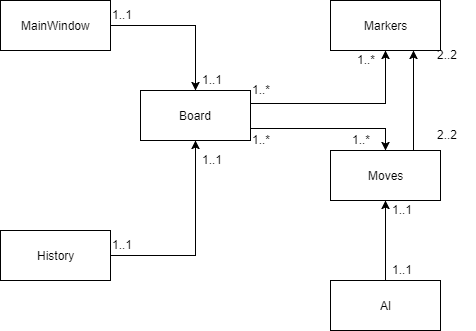
\includegraphics[scale = 0.4]{class-diagram}
  	\caption{Class Diagram- basic class diagram}
  	\label{fig:nonfloat}
	\end{figure}
To begin with six classes would be needed beginning with MainWindow.cs for the GUI, a Board class to build the board, a Marker Class to make each marker, an AI Class which would be implemented once a fully functional player vs player was completed, a History for storing games and a Move class to check for valid moves.This was later changed to incorporate extra features like the options menu and replay options window.

	\subsection{Board}
	\begin{figure}[H]
  	\centering
  	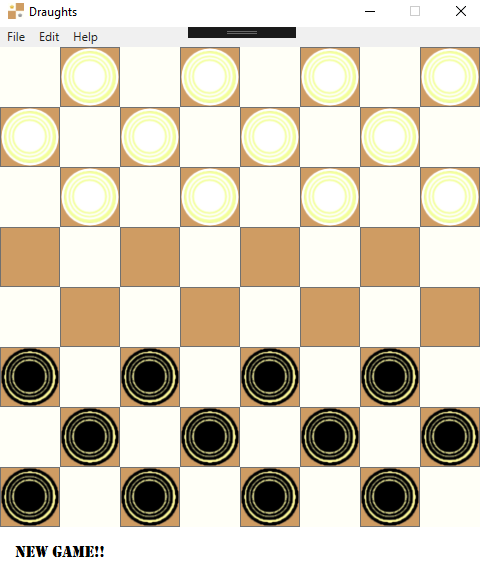
\includegraphics[scale = 0.4]{board}
  	\caption{Board and Markers - GUI of game board with markers ready to play}
  	\label{fig:nonfloat}
	\end{figure}

	To begin with the board was made using a 2D int array 8,8 so each square could be assigned to a number(-1 for invalid squares, 0 for empty squares, 1 White markers, 2 Black markers, 3 White kings, 4 Black kings) after the board was created in a text based environment and markers were placed using a the number system,it was at this point the decision to use a GUI would be a better representation for the game. The board was recreated in a GUI using stack-panels still with the same underlying numbering system. The empty board is created with buttons on the stack panels to allow the user to select them once marker are placed. The button is named with it row and column number.
	
	\subsection{Markers}
	The second stage of development moved on placing markers on the board a case statement was used to determine the placement of the markers, this is a more effective way to carryout the placement than the original way it was done in the text-based version which was a series of "if" statements. The markers are built using the Marker class which contains three values: the markers row and column and wither or not it has been promoted to a king. After placement is determined the marker gets added to the corresponding stack panel for that row and column, the button's name get updated with what the Marker colour is either black or white. An image of the marker is placed as the background of the button to show users what each button represents. Below is an image of the standard markers.
	\begin{figure}[H]
  	\centering
  	
\includegraphics[scale = 1.25]{Marker}
	\caption{Markers - game markers, White and Black Markers}
  	\label{fig:nonfloat}
	\end{figure}
	
	\subsection{Moves}
	The Move class  is used to create check move validation and checking if a jump move is available(take an opponents marker). Move validation is done by passing the marker colour to a method within the move class, It then checks to see if the placement chosen for the move is one column plus or minus one to the current column and plus a row for whites or minus a row for the blacks, this is done with four "if" statements. the other two check if the marker has a promotion and therefore can move up or down the rows regardless of colour. If the move is invalid a message box appears telling the user that it is invalid with a reason as to why.
	\begin{figure}[H]
  	\centering
  	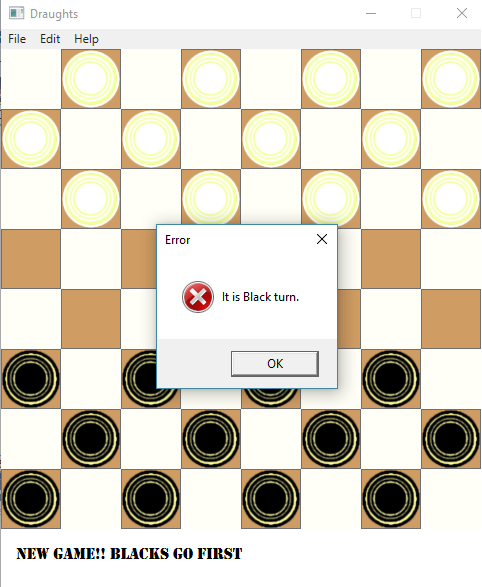
\includegraphics[scale = 0.5]{errors}
	\caption{Invalid move -message box showing error when moving a white marker of a black turn}
  	\label{fig:nonfloat}
	\end{figure}
	
	
Jumps validation is done using a series of if statements just like the move validation, but it checks two columns and plus or minus two rows depending on colour and promotion status. The jump possibilities get added to a list there if the list is populated a jump must occur.  

Promotions are dealt with in the MainWindow.cs in a KingMe method. that uses two "if" statements one for if the marker is "white" and the row is equal to eight. (bottom of the board for whites) or marker equal "black" and row equal to zero (top of the board for the blacks). If a marker is to be promoted the button name gets updated with the appropriate king either "WhiteKing" or "BlackKing" and the button's background image gets updated with the appropriate king image.
\begin{figure}[H]
  	\centering
  	
\includegraphics[scale = 1.25]{KingMarkers}
	\caption{Markers - game markers for promotion, White and Black King-Markers}
  	\label{fig:nonfloat}
	\end{figure} 
	\subsection{Player vs Player}
	Player vs Player (PVP) was done first to allow the game's logic to be fully tested therefore eliminating invalid moves that a player could make and therefore an AI player would not be-able to make as well. Making the game PVP first then adding AI allowed future features such as an undo feature to be added without impacting the games logic.  The winning condition is calculated by counting each players markers. and if any of the counts return a zero the other player wins.
	
	\subsection{Undo/Redo}
	To make the Undo/Redo Feature work I implemented four stacks. The undo feature uses Stacks after a player has preformed a move the move markers before and after position is added the a stack. if a marker was taken that markers co-ordinates re added to a taken marker stack so they can be replaced when a move is redone. The redo stack is added to after a move is undone and the retaken stack is added if piece that has been taken is replaced on the board.
	
	\subsection{AI}
	Lists and variation of the Fisher-Yates shuffle algorithm
	
	\subsection{Game Replay}
	uses 1 queue and 2 stacks 

	\section{Enhancements}
	extras:Background music, Player Names, keyboard shortcut, Game rules
	would like to have :AI VS AI, Game replays saved to a file for persistence
	
	\section{Critical Evaluation}
	x

	\section{Persona Evaluation}
	x
    
   
   


		
\end{document}